\chapter{Sviluppo ``BI Call Report'' per Azienda Acca Software}
\label{ch:Project}

A seguito del completamento dello studio svolto, riportato in precedenza, è stato svolto un incontro con i responsabili dei reparti interessati dell'azienda in modo da poter presentare e discutere riguardo gli argomenti trattati. Durante la riunione sono stati illustrati i punti salienti dello studio, mettendo in chiaro i pro e i contro di ogni aspetto analizzato. Tale presentazione ha permesso ai decision maker aziendali di comprendere, in linee generali, quali sono tutte le funzionalità, i sistemi e le possibilità che gli strumenti di \textit{Big Data}, \textit{Data Warehousing} e \textit{Data Analytics} possono portare all'interno di una compagnia. 

Una volta apprese le informazioni, è stato quindi svolto un'ulteriore riunione allo scopo di indicare l'obiettivo e le esigenze aziendali. Ciò ha permesso di iniziare la seconda parte della commissione, ovvero la progettazione e l'implementazione di una soluzione che permettesse di risolvere tutte le problematiche e di migliorare lo stato attuale dei processi aziendali. Il briefing ha avuto lo scopo di coinvolgere i vari partecipanti nell'attuazione del progetto, assegnando ruoli e responsabilità, definendo tempi e modalità, stabilendo indicatori di performance e criteri di valutazione.

Questo capitolo espone la fase di progettazione e implementazione del progetto. Lo scopo è fornire una panoramica generale del processo che ha portato alla definizione del progetto in questione, evidenziandone le motivazioni, le sfide e le opportunità che lo hanno caratterizzato ed ispirato.

\section{Definizione degli Obiettivi e dei Requisiti}

A seguito della presentazione svolta per mostrare tutte le possibilità del mondo dell'analisi dei dati è stato quindi compreso fin dal primo momento quale fosse il punto focalizzante dove l'azienda avrebbe dovuto puntare per migliorare nel proprio business, ovvero l'ambito del supporto tecnico fornito agli utenti. Quindi, per completare tale obiettivo è stato definito un progetto che avesse come fine il permettere al reparto di assistenza aziendale di migliorare dal punto di vista del supporto fornito, così da aumentare qualità ed efficienza dello stessp.

\subsection{Obiettivo del Progetto}

Fin dalla propria fondazione, Acca ha sempre messo al primo posto il rapporto con le persone, evitando che questo si limitasse alla mera interazione venditore-acquirente. L'azienda punta ad instaurare un rapporto di fiducia con i propri consumatori e per poter riuscire in tale compito la vendita di prodotti ad hoc pensati sulle loro esigenze non basta. È necessario permettere loro di risolvere ogni eventuale problema fornendogli un professionista del settore che sia capace di instradarlo verso la risoluzione di ogni possibile riscontro. Seguendo questa politica, la compagnia ha sempre fornito una produzione di software sulle necessità degli utenti associato ad un apposito servizio clienti che fosse capace di soddisfare ogni evenienza.

Proprio per questa motivazione, è stato scelto come obiettivo la definizione di un BPI che avesse lo scopo di migliorare la gestione delle chiamate che i clienti svolgono per essere aiutati, a seguito di essersi imbattuti in difficoltà che necessitassero dell'ausilio di appositi addetti messi a disposizione dall'azienda. Per riuscire in tale compito è stato ipotizzato fosse necessario un sistema che permettesse di raccogliere in modo approfondito quale fosse il flusso delle chiamate svolte (sia in uscita che in entranta) tra l'azienda e i propri clienti. Grazie al recupero di tali dati, sarebbe possibile applicare logiche di analisi sugli stessi in modo da comprendere eventuali difficoltà che il reparto di assistenza può incontrare; alcuni esempi sono la congestione del servizio offerto a seguito di una larga richiesta per determinati argomenti o giorni oppure comprendere quali siano i software che necessitano di maggiore assistenza.

In altri termini, l'obiettivo del progetto era quello di creare un sistema che permettesse il salvataggio centralizzato e strutturato di dati in modo che questi potessero essere analizzati dipendentemente dalle necessità (dinamiche) sorte in passato o che potrebbero sorgere in futuro.

\subsection{Analisi dei Requisiti}

Nel definire lo scopo ultimo, il progetto ha delineato l'idea cardine su cui fondare il tutto, tuttavia essa non è abbastanza, per iniziare un progetto è necessario definire in modo preciso cosa si vuole realizzare, perché, come e quali risorse si hanno a disposizione. Tale processo prende il nome di \textit{analisi dei requisiti} e consiste nell'identificare e poi documentare le caratteristiche e le funzionalità che lo stato finale del progetto dovrebbe avere.

L'\textbf{analisi dei requisiti} di un sistema è una metodologia strutturata per identificare un insieme appropriato di risorse che possa soddisfare le esigenze del sistema in questione e la definizione di requisiti per la progettazione o la selezione di tali risorse. I requisiti per un sistema o un elemento di un sistema sono descritti in una \textit{specifica}, ovvero una definizione precisa del progetto stesso. Perciò, l'analisi dei requisiti è il processo attraverso il quale è possibile ricavare una visione approfondita del contenuto corretto della specifica così definita \cite{system_requirements_analysis}.
La fase della specifica dei requisiti, essendo le fondamenta su cui il progetto si basa, è la più importante, dato che un errore può compromettere l'intero progetto. Per questo motivo la qualità di tale fase influisce in buona parte sulla qualità dell'intero prodotto finale. Perciò, scrivere una corretta \textit{specifica dei requisiti software} (o \textit{Software Requirements Specification, SRS}), ha un'importanza critica \cite{researchgate_srs_introduction}.

Non a caso, queste sono le parole di Frederick P. Brooks a riguardo\footnote{\textit{URL Fonte}: https://tinyurl.com/btyzuxkz}:

\begin{quote}
    «La parte più difficile del compito del software è arrivare a una specifica completa e coerente, e gran parte dell'essenza della creazione di un programma è infatti il debug della specifica.»
\end{quote}

La specifica deve essere sufficientemente chiara, non ambigua e non tecnica, tale che possa essere compresa anche da persone non facenti parte del mondo dello sviluppo software. Ciò rende possibile analizzare le richieste strutturate con criterio ed evitare possibili fraintendimenti su quest'ultime in modo che il prodotto finale possa soddisfare le richieste iniziali \cite{researchgate_srs_structure}.

\subsubsection{Definizione di Requisito}

Per chiarire maggiormente cosa si intende con il termine \textbf{requisito}, si riporta la definizione presente nel glossario di IEEE: «Una condizione o capacità che deve essere soddisfatta o posseduta da un sistema o da un componente del sistema per soddisfare un contratto, uno standard, una specifica o un altro documento formalmente imposto. L'insieme di tutti i requisiti costituisce la base per il successivo sviluppo del sistema o del componente del sistema.» \cite{software_requirements}. In altri termini, è possibile definire un requisito come una proprietà caratteristica di un sistema che ha lo scopo di risolvere una determinata problematica, riscontrata o eventualmente riscontrabile.

In generale, i requisiti di un sistema sono la combinazione di multipli requisiti provenienti da altrettante persone a diversi livelli di una compagnia o di ambito di interazione. Ciò, comporta che i requisiti varino nello scopo e nella proprietà che devono rispettare e per questo motivo si possono distinguere dipendentemente dal loro obiettivo in \cite{requirements_types}:

\begin{itemize}
    \item \textit{Requisito di prodotto}. Sono i requisiti derivanti da una necessità o un vincolo sul software da dover sviluppare (ad esempio, una funzionalità o simili).
    \item \textit{Requisito di processo}. Sono i requisiti derivanti da un vincolo sullo sviluppo del software in questione (ad esempio, l'adozione di una determinata tecnologia).
\end{itemize}

Inoltre, possono essere distinti in base alla tipologia di vincolo che impongono:

\begin{itemize}
    \item \textit{\textbf{Requisiti funzionali}}. Tali requisiti, anche conosciuti con il termine di \textit{capacità}, descrivono le funzionalità che il software deve fornire (risponde alla domanda ``cosa?''). Può essere descritto come un requisito per il quale è possibile scrivere un insieme finito di passaggi di test per poterne convalidare il comportamento.
    \item \textit{\textbf{Requisiti non funzionali}}. Tali requisiti, anche conosciuti con il termine di \textit{vincoli}, servono per vincolare la soluzione a rispettare determinate caratteristiche/qualità (risponde alla domanda ``come?''). Possono essere classificati a loro volta dipendentemente se facciano riferimento alla sicurezza, all'affidabilità, all'interoperabilità, alle prestazioni, alla compatibilità, e molte altri criteri.
\end{itemize}

\subsubsection{I Requisiti Funzionali del Progetto}

Di seguito sono riportati i requisiti funzionali definiti durante l'incontro:

\begin{itemize}
    \item \textbf{Acquisizione dei dati}. Il sistema dovrebbe essere in grado di acquisire dati da diverse fonti, compresi database, file di log e ulteriori sorgenti dove vengono originariamente salvati i dati.
    \item \textbf{Integrazione dei dati}. Il sistema dovrebbe permettere di integrare e consolidare dati provenienti da fonti differenti in un'unica struttura dati per garantire la coerenza e la completezza delle informazioni ricavate.
    \item \textbf{Archiviazione dei dati}. Il sistema dovrebbe fornire un meccanismo per l'archiviazione efficace e sicura dei dati, garantendo un accesso rapido ed efficiente.
    \item \textbf{Elaborazione dei dati}. Il sistema dovrebbe permettere l'esecuzione di operazioni di trasformazione, aggregazione e calcolo sui dati precedentemente archiviati per supportare analisi avanzate.
    \item \textbf{Storicizzazione dei dati}. Il sistema dovrebbe consentire la storicizzazione dei dati per analizzare l'evoluzione nel tempo delle metriche di assistenza tecnica, supportando in questo modo l'analisi di tendenza a lungo termine.
    \item \textbf{Ricerca dei dati}. Il sistema dovrebbe predisporre di funzionalità di ricerca per permettere agli utenti di trovare facilmente le informazioni di cui necessitano.
    \item \textbf{Interfaccia utente}. Il sistema dovrebbe fornire una interfaccia utente grafica (GUI) che consenta al personale preposto di accedere facilmente ai dati e alle analisi senza la necessità di competenze tecniche avanzate.
    \item \textbf{Generazione di report}. Il sistema dovrebbe permettere la creazione di report personalizzati sulle esigenze del personale che usufruisca del servizio.
    \item \textbf{Supporto di dashboard interattive}. Il sistema dovrebbe permettere la creazione di dashboard per monitorare in tempo reale le metriche chiave e facilitare la visualizzazione delle informazioni critiche.
\end{itemize}

\subsubsection{I Requisiti Non Funzionali del Progetto}
Di seguito sono riportati i requisiti non funzionali definiti durante l'incontro:

\begin{itemize}
    \item \textbf{Performance}. Il sistema dorebbe garantire prestazioni elevate durante l'interrogazione e l'elaborazione dei dati, anche in caso di volumi considerevoli.
    \item \textbf{Scalabilità}. Il sistema dorebbe essere progettato per gestire l'espansione dei dati nel tempo senza compromettere le prestazioni dello stesso.
    \item \textbf{Affidabilità}. Il sistema dorebbe assicurare una disponibilità elevata del sistema e la capacità di ripristinare i dati in caso di guasti o interruzioni.
    \item \textbf{Usabilità}. Il sistema dorebbe garantire un'interfaccia utente intuitiva e facile da usare in modo da ridurre al minimo il tempo di apprendimento per gli utenti.
    \item \textbf{Backup e ripristino}. Il sistema dorebbe essere predisposto per l'adozione di procedure per il backup regolare dei dati e garantire la possibilità dell'eventuale ripristino in caso di perdita dei dati.
    \item \textbf{Manutenzione}. Il sistema dorebbe fornire strumenti e procedure per la manutenzione regolare del sistema, inclusi aggiornamenti software.
    \item \textbf{Training degli utenti}. Il sistema dorebbe disporre della possibilità di usufruire di sessioni di formazione per garantire che gli utenti siano adeguatamente preparati per utilizzare il sistema in modo efficace.
    \item \textbf{Tempi di risposta}. Il sistema dorebbe permettere di svolgere interrogazioni e operazioni sui dati in tempistiche definibili accettabili, garantendo in questo modo un'esperienza utente fluida e reattiva.
    \item \textbf{Documentazione adeguata}. Il sistema dorebbe predisporre la presenza di una documentazione che sia sempre dettagliata e aggiornata sul sistema stesso (anche documentazione tecnica), cosi da semplificare la comprensione, manutenzione ed evoluzione del sistema nel tempo.
    \item \textbf{Manutenibilità}. Il sistema dorebbe essere facile da manutenere, con la possibilità di aggiungere o modificare funzionalità senza che il servizio venga interrotto.
\end{itemize}

Questi requisiti hanno portato all'identificazione di un sistema composto da due elementi principali, ovvero: un Data Warehouse, che si occupi di svolgere il compito della gestione dei dati, e un software di Business Intelligence, che si occupi della visualizzazione, interrogazione e la generazione di dashboard e report dai dati stessi.

\section{Studio sulla Raccolta dei Dati}

La raccolta dei dati rappresenta la fase cardine su cui fondare la riuscita di un sistema di DW e BI. Per sapere come strutturare l'intero progetto è stato quindi necessario svolgere un procedimento di studio rispetto alle sorgenti di dati fruibili. L'attuale capitolo fornisce un'analisi approfondita delle metodologie e delle considerazioni coinvolte nello studio sulla raccolta dei dati per il progetto in questione.

\subsection{Obiettivi dello Studio}

Lo scopo principale dello studio sulla raccolta dei dati è naturalmente quello di definire in modo chiaro quali sono i dati rilevanti su cui svolgere il processo di ETL. In altre parole, definire il modo corretto per estrarre, trasformare e infine caricare i dati all'interno del data warehouse. Più precisamente, sono stati identificati i seguenti obiettivi su cui lo studio doveva focalizzarsi:

\begin{enumerate}
    \item \textit{Identificare le fonti dei dati}. Determinare quali fossero le fonti dei dati, primarie e secondarie, pertinenti al reparto di assistenza tecnica.
    \item \textit{Definire la struttura dei dati}. Analizzare la struttura, il formato e lo schema dei dati presenti nelle fonti identificate nel passaggio precedente.
    \item \textit{Valutare la qualità dei dati}. Analizzare la qualità delle fonti di dati e dei dati stessi, identificando e affrontando le eventuali problematiche scaturite dalla possibile incompletezza, inaccuratezza o incongruenza.
    \item \textit{Determinare la frequenza di aggiornamento}. Definire la frequenza con cui i dati devono essere estratti e caricati all'interno del DW per garantire che le informazioni siano sempre aggiornate.
\end{enumerate}

\subsection{Metodologia di Raccolta dei Dati}
Una volta definiti gli obiettivi è stato quindi il momento di definire le metodologie che potessero portarli a termine.
\begin{enumerate}
    \item \textit{Analisi delle fonti di dati}. In questo caso si precisano quali sono le metodologie necessarie per comprendere al meglio le fonti dei dati su cui operare:
    \begin{itemize}
        \item File di log (fonti primarie). Analizzare i file di log generati da Asterisk\footnote{Asterisk è un'implementazione software di un sistema PBX (Private Branch Exchange), ovvero un server che gestisce la rete telefonica privata di un'organizzazione.} per comprendere le operazioni svolte dagli utenti e dagli operatori, in modo da conoscere le informazioni generate dalla fonte principali dei dati.
        \item Database (fonti primarie e secondarie). Esaminare i database dove vengono salvati tutti i dati generati dal reparto di assistenza, così da identificare le tabelle pertinenti, principali e non, i campi chiavi e le relative relazioni.
        \item Sistemi di ticketing e reporting (fonti secondarie). Scandagliare i sistemi di ticketing e reporting per acquisire informazioni ulteriori sui problemi segnalati, lo stato delle risoluzioni e i tempi di intervento, in modo da avvalorare i dati fondamentali con ulteriori informazioni.
    \end{itemize}
    \item \textit{Progettazione dell'estrazione dei dati}. In questa fase è necessario vagliare quali sono le metodologie da attuare per l'estrazione dei dati focalizzandosi sui seguenti punti:
    \begin{itemize}
        \item Identificazione dei campi chiave. Definire i campi chiave per ogni fonte dati per facilitare l'integrazione e l'identificazione univoca dei dati che si vogliono recuperare.
        \item Filtraggio dei dati. Implementare dei filtri necessari per estrarre solamente i dati necessari, riducendo la quantità di dati inutili da recuperare e gestire nel sistema di data warehouse.
        \item Strategia di caricamento incrementale. Stabilire una strategia di caricamento incrementale per ridurre il carico e i tempi, di estrazione dei dati così da poter garantire un aggiornamento dei dati rapido ed efficiente.
    \end{itemize}
    \item \textit{Valutazione della qualità dei dati}. In questo punto è necessario comprendere al meglio i dati e la loro qualità in modo da sapere come doverli gestire e a quali potersi affidare maggiormente o meno. In modo più approfondito, le tipologie di analisi della qualità dei dati sono le seguenti:
    \begin{itemize}
        \item Analisi dei dati mancanti. Identificare e trattare i dati mancanti attraverso tecniche di imputazione o altre soluzioni appropriate.
        \item Controllo di qualità. Implementare controlli di qualità per rilevare errori nei dati durante il processo di ETL.
        \item Standardizzazione dei dati. Applicare regole di standardizzazione per garantire coerenza nei formati dei dati.
    \end{itemize}
\end{enumerate}

Come è stato riportato nella fase di studio, una comprensione approfondita delle fonti dei dati, la progettazione accurata dei processi di ETL e la valutazione precisa della qualità dei dati così gestiti, sono punti fondamentali per garantire l'affidabilità e la pertinenza delle informazioni generate dagli stessi da parte del sistema. Per tale motivo, lo studio dei dati così proposto fornisce le basi per la messa in atto delle fasi successive di progettazione e conseguente implementazione del sistema di data warehouse e delle soluzioni di business intelligence.

\section{Progettazione di un Sistema di Data Warehouse}

La creazione di un sistema di data warehousing è un processo complesso che coinvolge diverse fasi chiave, dalla pianificazione iniziale alla progettazione, implementazione e manutenzione continua. Per questo motivo è utile suddividere tale compito definendo le fasi che lo compongono. Nel nostro caso, tenendo conto della definizione degli obiettivi del progetto già precedentemente svolta, le fasi adottate sono state le seguenti:
\begin{enumerate}
    \item Scelta dell'architettura del sistema di data warehouse.
    \item Progettazione del modello dei dati.
    \item Selezione delle tecnologie.
    \item Implementazione e caricamento dei dati.
\end{enumerate}

\subsection{Scelta dell'Architettura del Sistema}

Grazie alle conoscenze acquisite con lo studio teorico, è stato scelto di adottare un'architettura a due livelli in modo da avere una struttura solida, scalabile e performante ma allo stesso tempo non enormemente complessa se rapportata all'obiettivo del progetto.

Per avere una maggiore comprensione del tutto, si intende precisare che un sistema di data warehouse può essere suddiviso in modo generale in tre parti o livelli distinti, ovvero:

\begin{enumerate}
    \item \textit{Livello sorgente}. In tale livello sono situati tutte le fonti, eterogenee e non, da cui dover recuperare i dati da caricare all'interno del data warehouse.
    \item \textit{Livello del data warehouse}. In tale livello è presente il data warehouse vero e proprio dell'intero sistema, ovvero l'infrastruttura che si occupa di gestire i dati che si vogliono processare dalle fonti.
    \item \textit{Livello di analisi}. In tale livello sono presenti gli strumenti finali che si occupano di recuperare e gestire i dati ad alto livello per metterli a disposizione degli utenti finali.
\end{enumerate}

Un'architettura a uno, due o tre livelli identifica il numero di sottolivelli che caratterizzano il secondo livello, ovvero quello del DW. Nel nostro caso, adottando un'architettura a due livelli, esso viene suddiviso in un \textit{livello di alimentazione} e un \textit{livello di data warehouse}. Il primo sottolivello si occuperà di svolgere le operazioni di processamento dei dati, mentre il secondo si occuperà di salvare tutti i dati supportato da un contenitore di metadati. Nel nostro sistema è stato scelto di non adottare dei data mart poiché il progetto è momentaneamente ristretto ad un solo ambito di utilizzo e applicazione e quindi la scelta di aggiungerli avrebbe aumentato la complessità del progetto senza apportare alcun miglioramento o beneficio. Invece, il contenitore di metadati avrà un ruolo cruciale, come nella maggior parte dei sistemi, poiché avrà il compito di mantenere le informazioni sulle sorgenti, sui meccanismi di accesso, sulle procedure di pulitura, trasformazione e alimentazione, ecc.

\subsection{Progettazione del Modello dei Dati}

Tale fase è cruciale per la riuscita di un sistema di data warehousing poiché coinvolge la definizione di come i dati debbano essere strutturati all'interno del sistema e quindi come essi possano essere sfruttati per sopperire alle esigenze di analisi e reporting dei dati da parte degli utenti finali.

Come primo dubbio bisogna risolvere la scelta tra uno schema dimensionale oppure uno schema normalizzato. A tal proposito di seguito sono riportati i vantaggi e gli svantaggi riscontrati nell'analizzare entrambe le possibili scelte:

\begin{itemize}
    \item \textit{Schema Dimensionale}:
        \begin{itemize}
            \item Vantaggi:
                \begin{itemize}
                    \item Facilita le query analitiche complesse.
                    \item Semplifica la comprensione e navigazione per gli utenti finali.
                \end{itemize}
            \item Svantaggi:
                \begin{itemize}
                    \item Richiede maggiore spazio di archiviazione.
                \end{itemize}
        \end{itemize}
    \item \textit{Schema Normalizzato}:
            \begin{itemize}
            \item Vantaggi:
                \begin{itemize}
                    \item Minimizzazione della ridondanza dei dati.
                    \item Risparmio di spazio di archiviazione.
                    \item Manutenzione semplificata dei dati.
                \end{itemize}
            \item Svantaggi:
                \begin{itemize}
                    \item Maggiore complessità delle query analitiche.
                \end{itemize}
        \end{itemize}
\end{itemize}

Date queste analisi è stata scelta la seconda ipotesi, ovvero lo schema normalizzato, poiché il più affine rispetto alle seguenti scelte già preventivate:

\begin{enumerate}
    \item L'utente finale dovrà avere accesso unicamente al DSS messo a disposizione per svolgere analisi e report. Tale scelta comporta che qualsiasi complessità il sistema di data warehouse interno possa avere, esso dovrà essere completamente astratto rispetto al livello di presentazione adoperato degli utenti finali.
    \item È molto probabile che il sistema venga arricchito con ulteriori dati provenienti da fonti tuttora non considerate e per questo motivo necessiterà di manutenzione ed aggiornamento. Tale scelta implica che l'eventuale utilizzo dello schema dimensionale possa comportare una maggiore difficoltà nella manutenzione ed aggiornamento.
    \item Per permettere una migliore interoperabilità con ulteriori futuri data mart da integrare nel data warehouse, oppure ulteriori utilizzi differenti da quello attualmente ipotizzato, mantenere i dati il meno ridondanti possibili e maggiormente uniformati è un importante compito ed obiettivo.
\end{enumerate}

\subsection{Selezione delle Tecnologie}

Come seconda fase è stato necessario scegliere quali tecnologie si volessero adottare per l'implementazione del sistema. Sono diverse le tecnologie coinvolte nelle fasi di estrazione, trasformazione e caricamento (ETL), nella gestione del database di data warehouse e nelle attività di business intelligence. Più precisamente:

\begin{enumerate}
    \item \textit{Strumenti di ETL}. Come strumento di ETL è stato adottato uno strumento custom implementato ad hoc per tale compito. È stato preferito a degli strumenti messi a disposizione dal mercato attuale (dove i più comuni sono \textit{Talend}, \textit{Apache NiFi} e \textit{Microsoft SSIS}) per motivi di massima personalizzazione in base alle esigenze aziendali.
    \item \textit{DBMS per il Data Warehouse}. Come DBMS per la gestione dei dati del sistema è stato adottato PostgreSQL, un database SQL relazionale. È stato preferito a database come \textit{Amazon Redshift}, \textit{Snowflake} o \textit{Google BigQuery} poiché per il momento l'azienda ha deciso, per questioni di privacy e sicurezza, di adottare soluzioni che permettessero di mantenere i dati all'interno della stessa. Tuttavia, se in futuro si decidesse di voler espandere le dimensioni e la complessità del progetto, sarà facilmente possibile adottare una soluzione come Amazon Redshift essendo quest'ultimo basato proprio su PostgreSQL.
    \item \textit{Strumenti di Business Intelligence}. Come strumento DSS per la BI è stato adottato \textit{Power BI}, tra gli strumenti attualmente in commercio (altri sono \textit{Tableau}, \textit{Looker} o \textit{Datapine}). Tale scelta è dovuta dal fatto che è uno degli strumenti utilizzati da maggior tempo e con maggiore diffusione. Ciò permette di avere un software con aggiornamenti garantiti e sempre nuove funzionalità, aggiornabili anche aggiungendo add-on custom, aumentando le possibilità del progetto stesso.
\end{enumerate}

Tali scelte sono state ponderate avendo preso in considerazione le seguenti motivazioni:
\begin{itemize}
    \item \textit{Compatibilità con l'infrastruttura esistente}. Le tecnologie selezionate si integrano facilmente con l'infrastruttura IT esistente per garantire una transizione fluida.
    \item \textit{Scalabilità}. Le tecnologie sono in grado di scalare per gestire crescenti volumi di dati e carichi di dati, in termini accettabili tali da sopperire alla possibile evoluzione del progetto.
    \item \textit{Facilità di utilizzo}. Gli strumenti e le piattaforme sono intuitivi e facilmente utilizzabili dagli utenti finali, riducendo la necessità di formazione estensiva.
    \item \textit{Prezzo e licenza}. Il \textit{costo totale di proprietà} (TCO) delle tecnologie, compresi i costi di licenza, di implementazione e di manutenzione continua sono nulli o minimi rispetto ad una possibile evoluzione del servizio.
    \item \textit{Supporto della community e aggiornamenti}. Le tecnologie godono di un supporto attivo dalla community o dal fornitore e ricevono aggiornamenti regolari per rimanere al passo con le nuove tecnologie e correggere eventuali vulnerabilità.
    \item \textit{Facilità di Manutenzione}. Le tecnologie sono di facile gestione e manutenzione agevole per garantire un funzionamento continuo del sistema.
\end{itemize}

\section{Processo di ETL}

\subsection{Analisi del Processo di ETL}

Una volta preso atto delle risorse aziendali è quindi necessario delineare il processo di ETL per la gestione dei dati. Per quanto spesso sia dato per scontato, questo compito non va sottovalutato, anche esso è un punto cruciale per la riuscita di un sistema di data warehousing. Come accennato in precedenza, questa fase si occupa di estrarre i dati dalle fonti originali, trasformarli in un formato adatto per l'analisi, e caricarli nel data warehouse. Di seguito si approfondiscono tutti i passaggi del processo di ETL:

\begin{enumerate}
    \item \textit{Estrazione}. La fase di estrazione, che si occupa del recupero dei dati dalle varie fonti messe a disposizione, è caratterizzata da:
    \begin{itemize}
        \item Tecniche. Sono di due tipi: \textit{estrazione completa}, che recupera ogni volta l'interezza dei dati della fonte, ed \textit{estrazione incrementale}, che recupera solo i dati nuovi, modificati o che in precedenza sono stati evitati.
        \item Metodologie. Esistono differenti tipologie di estrazione, le più comuni sono: esecuzione di \textit{query sui database}, scraping\footnote{Per \textit{scraping dei dati} (o semplicemente \textit{scraping}) si intende una tecnica in cui un programma informatico estrae dei dati dall'output generato da un altro programma.} dai \textit{file di log} e effettuare \textit{richieste API} alle fonti che le espongono.
    \end{itemize}
    \item \textit{Trasformazione}. La fase di trasformazione, che si occupa del convertire i dati estratti in formati coerenti e facili da gestire, è caratterizzata da:
    \begin{itemize}
        \item \textit{Attività}. Le principali attività di trasformazione riguardano la \textit{pulizia}, la \textit{standardizzazione}, l'\textit{arricchimento} e l'\textit{aggregazione} dei dati recuperati.
        \item \textit{Linguaggio}. Il linguaggio di programmazione adottato nello svolere le attività elencate permette di essere più efficiente o semplice, dipendentemente dalla caratteristica che si ricerca.
        \item \textit{Strumenti}. Per riuscire in tale compito, è possibile adottare strumenti che permettono renderlo più semplice, intuitivo o immediato.
    \end{itemize}
    \item \textit{Caricamento}. La fase di caricamento o salvataggio, che si occupa di inserire i dati trasformati all'interno del data warehouse, è caratterizzata da:
    \begin{itemize}
        \item Metodologie. Quando si parla di metodologia di caricamento si fa riferimento alla possibilità di scegliere se caricare i dati in un formato \textit{batch}, ovvero caricati periodicamente a lotti, oppure in \textit{tempo reale}, inserendo ogni volta il singolo record recuperato e gestito.
        \item Approcci. In questo caso, per approccio al caricamento si intende il modo in cui si intende svolgerlo, ovvero se svolgere un \textit{caricamento completo} inserendo i dati solo quando tutti i dati sono stati estratti e trasformati, oppure se svolgere un \textit{caricamento incrementale} inserendo i dati  quando vengono gestiti volta per volta.
    \end{itemize}
\end{enumerate}

\subsection{Definizione delle Caratteristiche del Processo di ETL}

Date le caratteristiche sopracitate e le risorse messe a disposizione dall'azienda è stato necessario creare un sistema personalizzato che svolgesse il processo di ETL. Tale motivazione ha portato ad adottare un linguaggio di programmazione come Golang per scrivere il codice che si occupasse di tale compito. La scelta è ricaduta sul linguaggio ideato da Google poiché è efficiente, stabile e allo stesso tempo non complesso da adottare. Quindi in un'ottica di scalabilità del progetto, oppure di ampliamento del team ad ulteriori persone, con la giusta documentazione, tale compito non comporterebbe una elevata difficoltà. Inoltre, tale programma, una volta completo, è stato caricato all'interno di un'immagine docker per poi essere hostato da un server aziendale in un container apposito, tale che le funzionalità predisposte siano sempre a disposizione degli utenti finali.

Il programma così creato si occupa di svolgere l'intero processo di ETL in modo iterativo ogni minuto, in modo da avere sempre dati aggiornati all'interno del data warehouse. Tale scelta, ha però comportato la necessità di dover gestire la possibilità di incontrare stati dei record incompleti o incongruenti, dato che l'aggiornamento delle risorse originali non viene svolto in modo sincronizzato. Per poter gestire tale problematica, il sistema oltre a caricare i dati in modo incrementale, in modo da non dover sempre gestire un alto carico di dati e da non sforzare le risorse nell'estrarre i dati, si occupa di caricare ogni volta le informazioni basilari recuperabili dalle fonti, per poi aggiornarle in un'iterazione successiva al recupero dei dati ulteriori da dover inserire per completare l'intero record finale. In questo modo, viene rimossa ogni possibilità di incongruenza o perdita dei dati che necessitasse che tutte le risorse avessero i dati al loro interno in contemporanea. Quindi, il sistema si occupa, ad ogni iterazione, di recuperare le informazioni da multiple fonti differenti (sia file di log che database) per poi svolgere operazioni di pulizia e formattazione, in modo da svolgere operazioni di caricamento incrementale e batch. La possibilità di far coincidere la metodologia e l'approccio di caricamento sopracitati è dovuta proprio al fatto che le iterazioni vengono svolte a poca distanza l'una dall'altra e per questo motivo i dati da gestire sono pochi ed un caricamento batchato comporta la necessità di dover svolgere un numero minore di operazioni senza che queste siano troppo pesanti.

\subsection{Motivazioni delle Decisioni Implementative}

Nel decidere quali approcci o caratteristiche adottare nel nostro sistema, sono state prese in considerazione le seguenti motivazioni:
\begin{itemize}
    \item \textit{Controllo di qualità dei dati}. Il sistema implementa controllo di qualità per garantire l'integrità e l'accuratezza dei dati rimuovendo ogni possibile refuso, dati che presentano formati contrastanti o errati, oppure dati che si compongono principalmente di informazioni che non risulterebbero necessarie o addirittura fuorvianti.
    \item \textit{Gestione degli errori}. Il sistema prevede meccanismi per gestire e registrare gli errori durante l'intero processo, insieme ad un sistema di logging, in modo da poter individuare immediatamente il problema e risolvere il tutto.
    \item \textit{Pianificazione e scheduling}. Con una corretta pianificazione e scheduling delle iterazioni che il sistema deve svolgere, è possibile definire le migliori finestre temporali predeterminate in modo da evitare impatti sulle comuni operazioni aziendali oppure aumentare o diminuire il tempo di differimento tra una esecuzione e un'altra in base alle necessità.
    \item \textit{Monitoraggio delle prestazioni}. Il programma permette di avere, anche grazie al sistema di logging interno sopracitato, la possibilità di monitorare le prestazioni dello stesso, in modo da poter comprendere se siano presenti dei rallentamenti in determinate attività svolte durante il processo di ETL, oppure se siano congestionate le risorse in quel momento.
    \item \textit{Gestione delle modifiche}. Il sistema mette a disposizione, degli operatori del settore, di modificare nel tempo le scelte delle attività da dover svolgere, in modo da permettere una personalizzazione approfondita e perfetta per le necessità mostrate degli utenti finali.
\end{itemize}

\section{Creazione di Dashboard e Report Finali}

\subsubsection{Scelta del DSS}

Una volta predisposto il data warehouse e creato il sistema che si occuperà del processo di ETL, è ora necessario adottare un sistema di DSS in modo da poter mettere a disposizione i dati agli utenti finali. Per riuscire in tale compito, è stato deciso di adottare il software di casa \textit{Microsoft} ``\textbf{Power BI}''. 

Come accennato in precedenza, tale scelta è dovuta alla grande importanza del software in questione nel mondo della Business Intelligence data l'ampia diffusione dello stesso. Tuttavia, il suo largo utilizzo e la sua sempre attiva community non sono le uniche motivazioni che hanno valorizzato la scelta. Il software in questione dispone sia di un'interfaccia Web sia di un'interfaccia desktop, da utilizzare offline, leggere e user-friendly. Questa doppia valenza, ci permette di strutturare il progetto dal punto di vista del livello più esterno in due fasi distinte, ovvero: 

\begin{enumerate}
    \item Una prima fase che limiterà l'utilizzo del software ``\textit{Microsoft Power BI Desktop}'' solamente agli utenti preposti ai quali sarà messa a disposizione l'applicazione e il file con all'interno le dashboard e i report creati. Ciò permetterà di mantenere un accesso controllato e limitato ai soli utenti principali adottando account personali per la visualizzazione delle informazioni.
    \item Una seconda fase che permetterà l'accesso all'interfaccia di reportistica tramite l'ausilio della piattaforma web hostando il tutto in un server interno grazie all'adozione del servizio ``\textit{Server di report di Power BI}''. Ciò permetterà di espandere l'accesso ad ulteriori utenti e tenerlo allo stesso tempo controllato, in modo da mantenere un servizio stabile e scalabile.
\end{enumerate}

\subsection{Caratteristiche delle Dashboard e Report da Creare}

La fase finale del progetto comprende l'unica parte di cui un utente finale ha visione e maggiore interesse. Proprio per tale motivo, riuscire a definire delle dashboard o report è un aspetto molto importante, poiché da questo dipenderà la facilità di comprensione e interattività con i decision maker. Per poter completare al meglio tale compito, è stata varata l'analisi dei seguenti punti:

\begin{enumerate}
    \item \textit{Definizione degli obiettivi}. Arrivati a questo punto è stato necessario approfondire con gli utenti finali quali fossero i KPI e i dati di loro interesse. Per tale motivo è quindi stato necessario definire le domande chiave che gli utenti avevano necessità di risolvere e gli obiettivi di business dell'organizzazione, così da poter delineare le dashboard e i report in base ai relativi bisogni.
    \item \textit{Progettazione dell'interfaccia utente}. Questa fase, grazie all'utilizzo di Power BI come software DSS permette di essere parzialmente completa in partenza necessitando di una progettazione dell'interfaccia solo per quanto riguarda le dashboard e i report utilizzabili. Per questo motivo, per tutte le dashboard e report è stato definito un design comune che permettesse agli utenti di familiarizzare con lo stesso e non dover approcciare ad un layout differente ad ogni interrogazione differente.
    \item \textit{Selezione delle visualizzazioni}. Mettendo alla base di questo punto la definizione degli obiettivi e dell'interfaccia delle fasi precedenti, è stato necessario comprendere quali fossero i grafici e i diagrammi che meglio si sarebbero adattati alle necessità mostrate. Per creare un'interfaccia user-friendly, è stato scelto di adottare un insieme di grafici eterogeneo ma dal numero non elevato. Ciò ha permesso di non diminuire la facilità di utilizzo, che con un numero troppo elevato di differenti grafici ne sarebbe risultata compromessa, e allo stesso tempo ha permesso di visualizzare i dati in modo efficiente senza limitazione alcuna.
    \item \textit{Creazione di dashboard}. A seguito della definizione dei grafici da adottare nel sistema, è stato quindi possibile delineare quali dovessero essere le dashboard principali e secondarie. Permettendo in questo modo di suddividere e mettere in primo piano le panoramiche generali nelle dashboard principali, aventi al loro interno le metriche e i KPI chiave, e le informazioni settoriali nelle dashboard secondarie, contenenti metriche focalizzate su determinati ambiti o settori così da permetterne un approfondimento degli stessi.
    \item \textit{Creazione di report}. Lo strumento Power BI è stato adottato anche per la sua duttilità, permettendo di essere adoperato sia per la creazione di dashboard sia per la creazione di report. In questo caso, sono stati definiti i report operativi e analitici che permettessero di fornire dettagli specifici sulle attività e le prestazioni del reparto, così da permettere ai decision maker di esplorare in modo approfondito i dettagli degli stessi.
\end{enumerate}

Naturalmente, nel progettare le dashboard messe a disposizione, è stato sempre messo in conto la caratteristica principale della possibilità di permettere un'interattività diretta e responsiva tra l'utente e il DSS contente i dati in questione.

\subsection{Definizione delle Dashboard e dei Report}
Nel suddetto percorso verso l'implementazione della fase finale di un sistema di Business Intelligence, la compagnia ha affrontato l'importante decisione di definire la strategia di presentazione dei dati. Tale strategia ha così permesso di delineare quali fossero gli obiettivi e le modalità con cui si volessero raggiungere. La scelta è stata di seguire un piano incentrato principalmente sull'adozione di report e con alcune dashboard che potessero supportare gli stessi.

La scelta di dare priorità all'implementazione di pagine di report è stata guidata da diverse considerazioni chiave. La natura complessa e articolata delle informazioni da poter ricavare dalle attività svolte dal reparto di supporto tecnico e le enunciate necessità di analisi approfondite hanno richiesto una presentazione dettagliata e tecnica di tutti i dati. Essendo i report, pagine di raccolta dati che fanno delle tabelle il loro punto cardine, hanno mostrato una maggiore affinità con le necessità aziendali. I report permettono agli utenti finali di svolgere un monitoraggio, preciso, conciso e dettagliato allo stesso tempo di tutti i dati gestiti dal sistema di data warehousing, in particolare fornendo informazione relativi a (1) telefonate ricevute, (2) feedback da parte dei clienti rispetto alla qualità delle risposte degli operatori e (3) report complessivo. Le analisi svolgibili sui report permettono una maggiore facilità nel comprendere i dati in visione, l'identificazione chiara e veloce delle aree di interesse e soprattutto la valutazione delle metriche chiave di cui si vuole tenere traccia. Tuttavia, per cercare di rendere il tutto maggiormente intuitivo, rapido e semplice, l'azienda ha comunque deciso di comprendere nel sistema di BI delle pagine di dashboard che potessero rappresentare e riassumere velocemente tutte le informazioni riportate minuziosamente nei report. Per tale motivo, alcune dashboard sono state sviluppate per fornire una visione sintetica e immediata delle suddette metriche chiave. In questo modo, l'adozione di entrambe le tipologie di presentazione dei dati ha permesso agli utenti finali di avere uno strumento onnicomprensivo che gli permettesse di soddisfare sia bisogni maggiormente specifici sia semplicemente sintetici.

Le Figure \ref{fig:BI Call Report-1}, \ref{fig:BI Call Report-2}, \ref{fig:BI Call Report-3} e \ref{fig:BI Call Report-4} riportano rappresentazioni visive delle dashboard create e dei parametri presi in considerazione per ottenere i report finali. È importante sottolineare che i dati riportati nelle Figure mostrate sono dati fittizzi puramente a titolo illustrativo, poiché i dati reali sono coperti da privacy e proprietà intellettuale di Acca Software. Di seguito, sono riportate le caratteristiche individuate per ogni categoria (e singolo report o dashboard):

\begin{enumerate}
    \item \textbf{Analisi dei dati generali}.   
        \begin{itemize}
            \item \textit{Telefonate totali}. Tale pagina  è un report che permette di analizzare tutti i valori puntuali e medi giornalieri (suddivisi per mese o anno) delle telefonate ricevute dal reparto di supporto, con metriche di analisi percentuale ed effettiva rispetto alle richieste fatte. 
            \item \textit{Telefonate Totali (Grafici)}. Tale pagina è una dashboard riassuntiva del precedente report, che ha lo scopo di sintetizzare l'andamento generale delle chiamate ricevute nell'arco del periodo in esame.
            \item \textit{Telefonate Gestite (IN/OUT)}. Tale pagina è un report che permette di analizzare tutti i valori puntuali e medi giornalieri (suddivisi per mese o anno) delle telefonate gestite, ovvero le telefonate per cui è stato fornito un servizio di assistenza (sia in uscita che in entrata), con metriche di analisi percentuale ed effettiva rispetto alle richieste fatte.  
        \end{itemize}
    \begin{figure}[H]
    \centering
    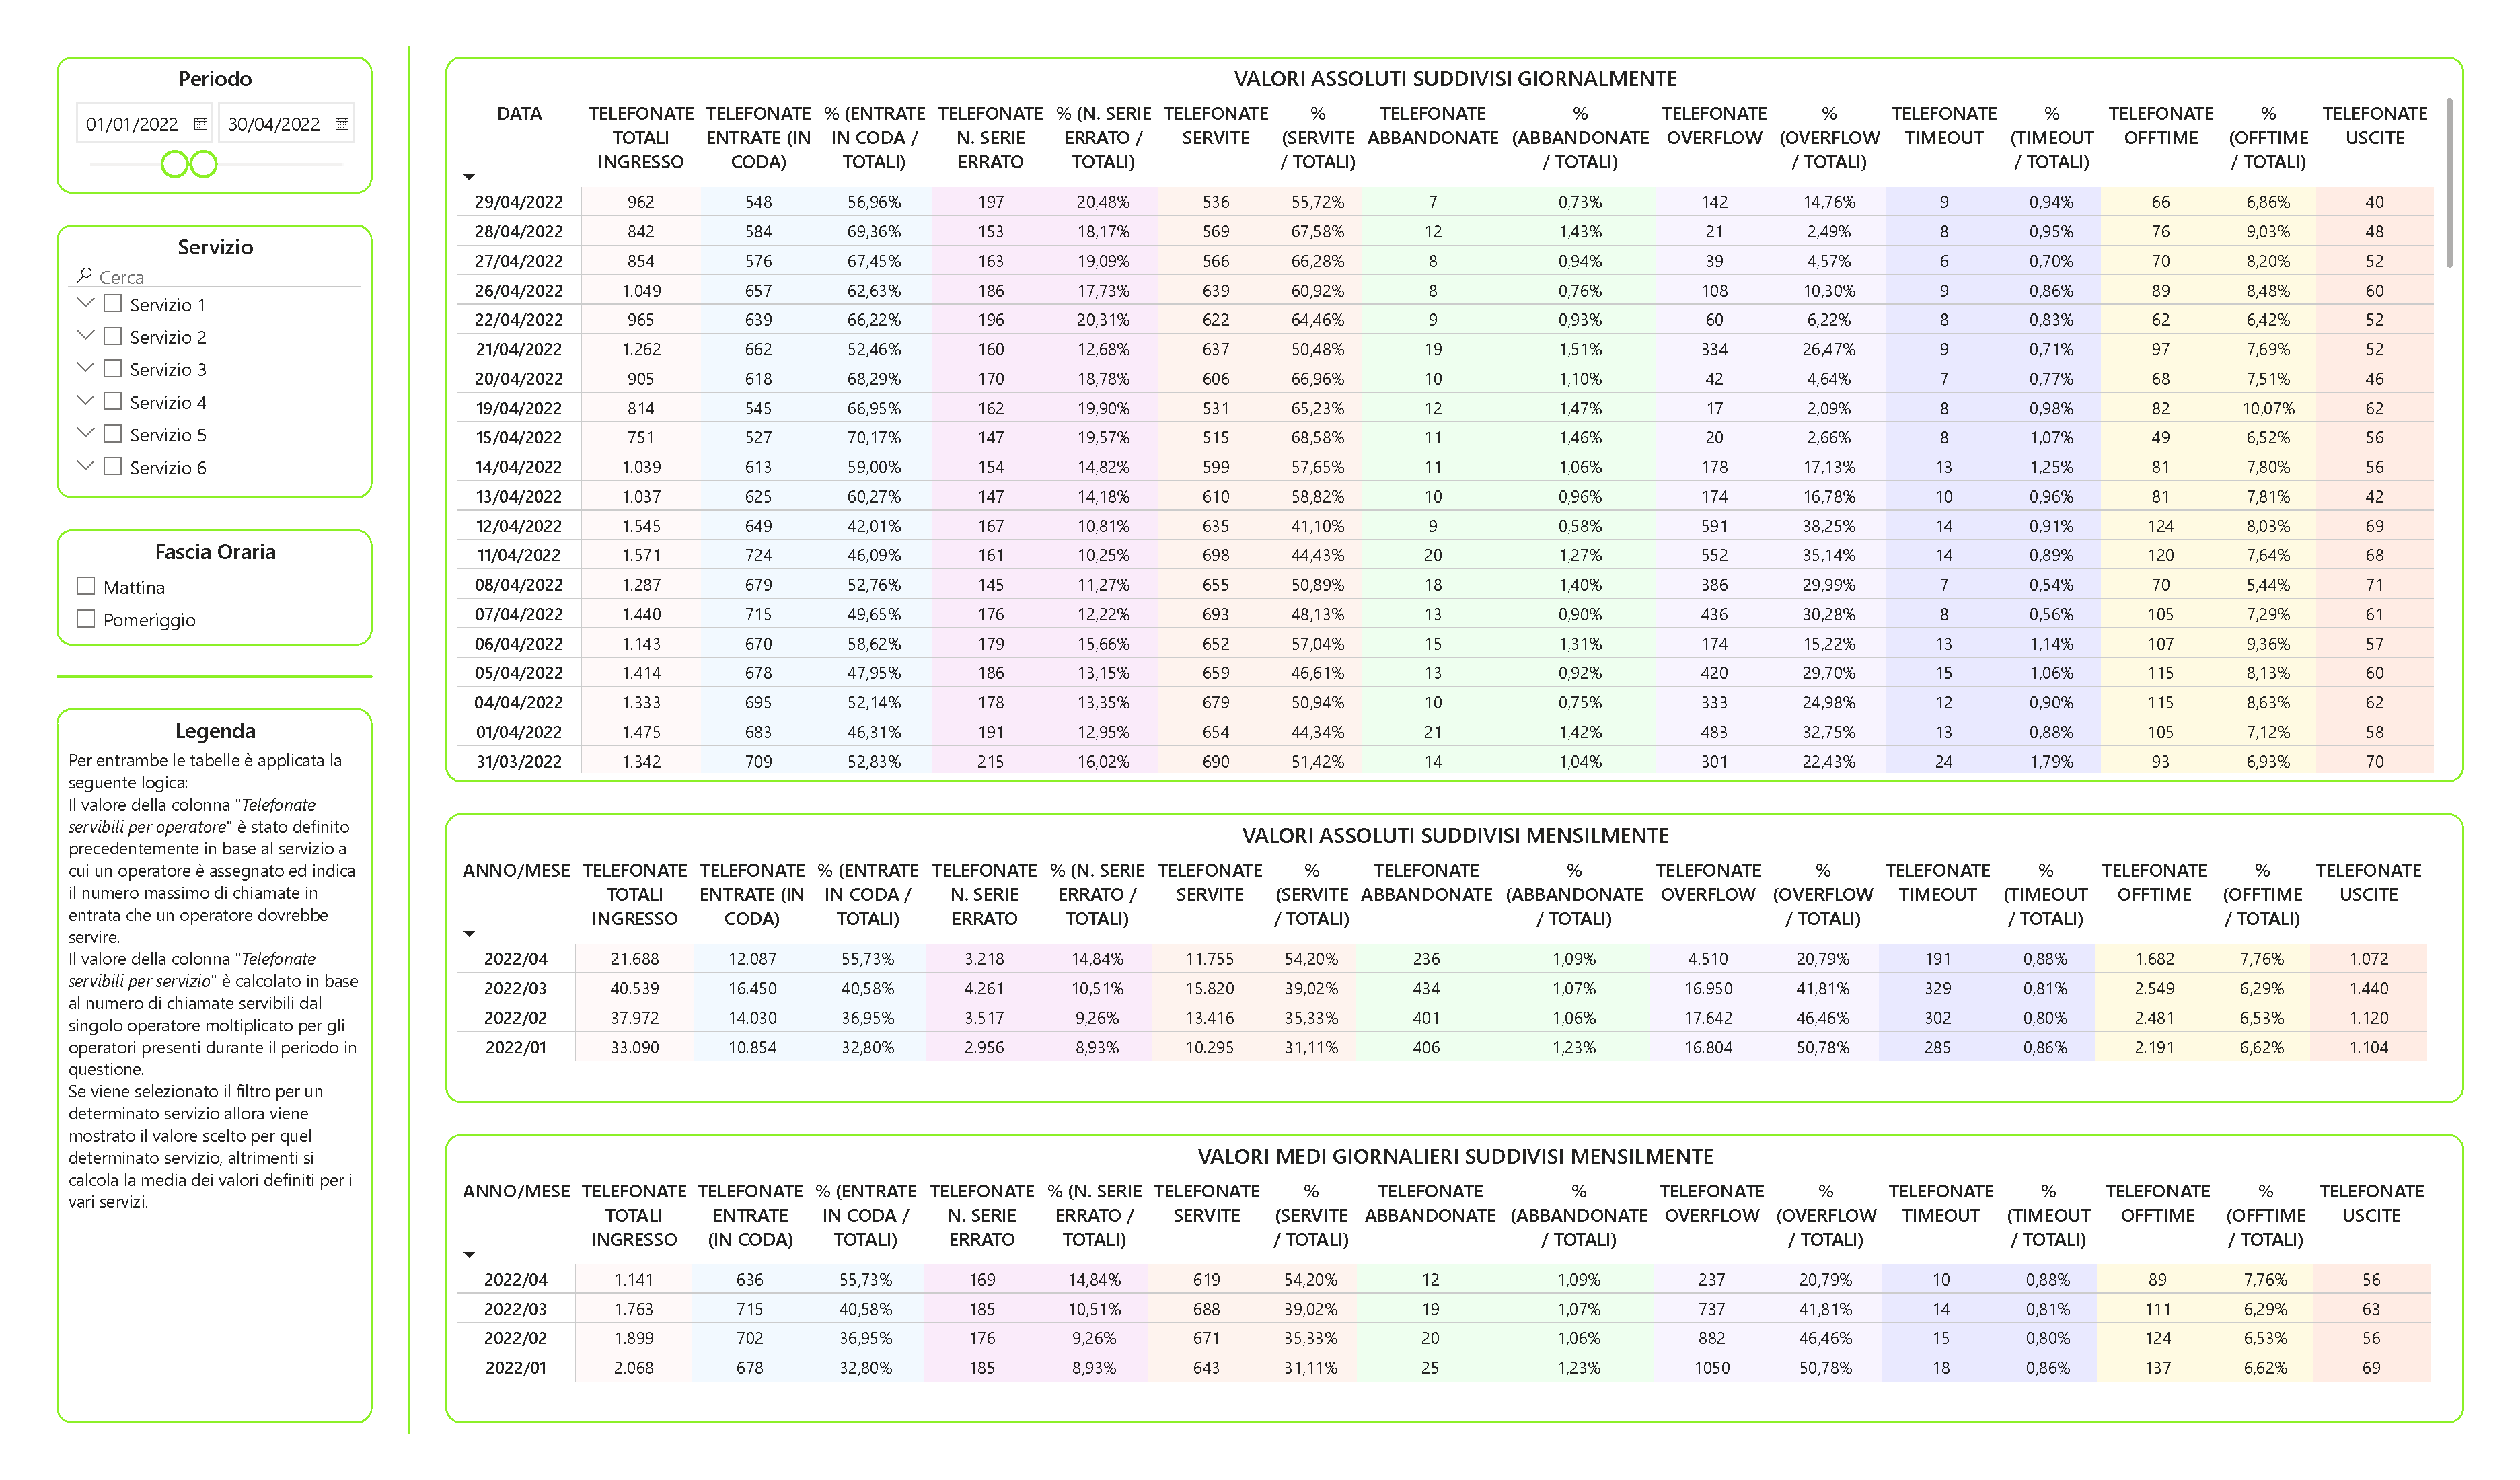
\includegraphics[width=1\linewidth]{figure/capitolo_4/BI Call Report-1.pdf}
    \caption{Telefontate Totali}
    \label{fig:BI Call Report-1}
    \end{figure}
    \item \textbf{Analisi della qualità dei servizi offerti}.
        \begin{itemize}
            \item \textit{Confronto operatore}. Tale pagina è un report che permette di analizzare l'andamento medio giornaliero rispetto alle telefonate gestite da ogni operatore facente parte del reparto, con possibilità di analizzare la tipologia di supporto e le relative valutazioni se rilasciate dai clienti.
            \item \textit{Analisi Feedback}. Tale pagina è un report che permette di visualizzare in modo oculato ogni feedback rilasciato dai clienti, con annesse informazioni rispetto all'operatore che si è occupato della chiamata e del software per cui è stato svolto il supporto.
            \item \textit{Feedback Ricevuti}. Tale pagina è un report che permette di analizzare tutti i valori puntuali e medi giornalieri (suddivisi per mese o anno) dei feedback rilasciati dai clienti rispetto alle chiamate per cui hanno ricevuto assistenza.
        \end{itemize}
        \begin{figure}[H]
        \centering
        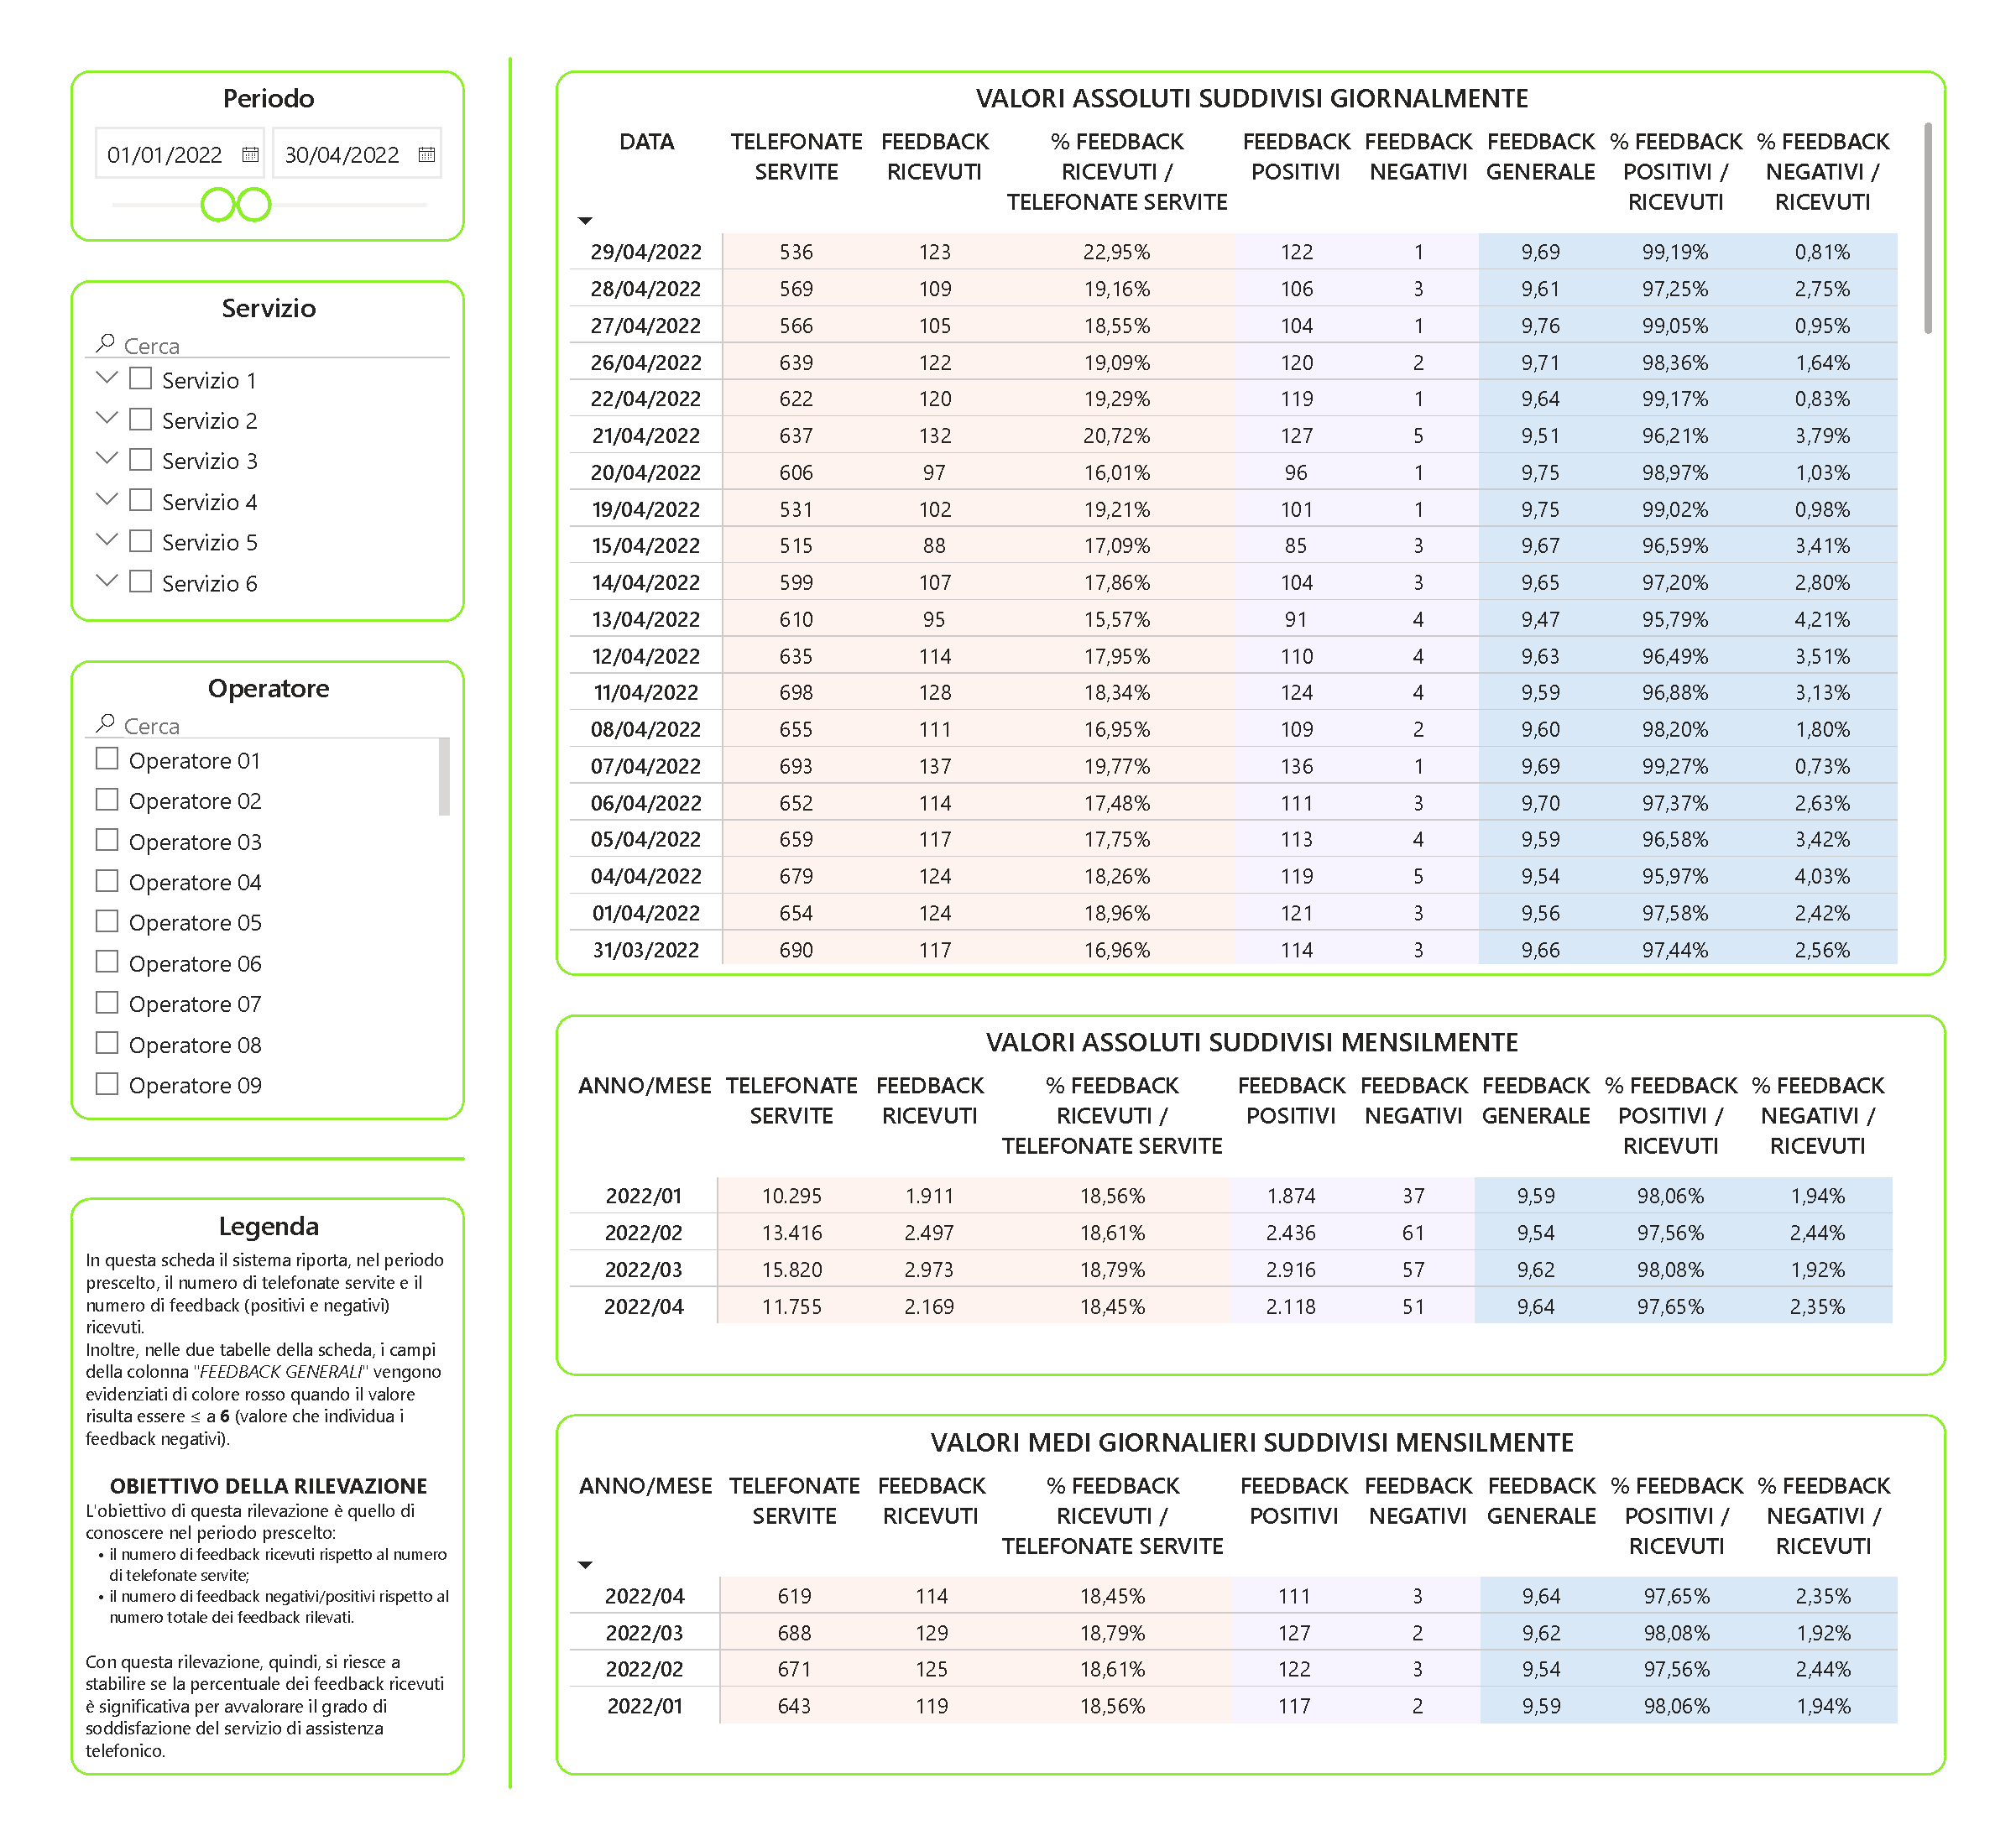
\includegraphics[height=0.8\linewidth]{figure/capitolo_4/BI Call Report-2.pdf}
        \caption{Feedback Ricevuti}
        \label{fig:BI Call Report-2}
        \end{figure}
        \item \textbf{Analisi dell'andamento dei servizi}.
        \begin{itemize}
            \item \textit{Gestite (Servizi/Software)}. Tale pagina include sia una sezione di dashboard sia una sezione di report per permettere di prendere visione in modo sintetico e preciso di tutti i dati relativi alle telefonate gestite dal reparto suddivise rispetto al servizio o al software che si vuole analizzare.
            \item \textit{Andamento (Servizi/Software)}. Tale pagina è una dashboard a supporto del report precedente, che ha il compito di permettere di paragonare periodi differenti per un medesimo servizio o software e comprenderne la differenza di andamento.
            \item \textit{Servite (dal 2013)}. Tale pagina include sia una sezione di dashboard sia una sezione di report per permettere di prendere visione in modo sintetico e preciso di tutti i dati relativi alle telefonate gestite dai vari servizi suddivisi in anni, con dati integrati a quelli recuperati dal DW, in modo da avere un quadro completo dell'andamento puntuale con il passare del tempo.
            \item \textit{Servite (grafico lineare)}. Tale pagina è una dashboard con il compito di riassumere l'andamento delle telefonate, suddivise per settimane lavorative, rispetto ai servizi dal massimo periodo che è possibile prendere in analisi recuperando i dati dal data warehouse.
        \end{itemize}
        \begin{figure}[H]
        \centering
        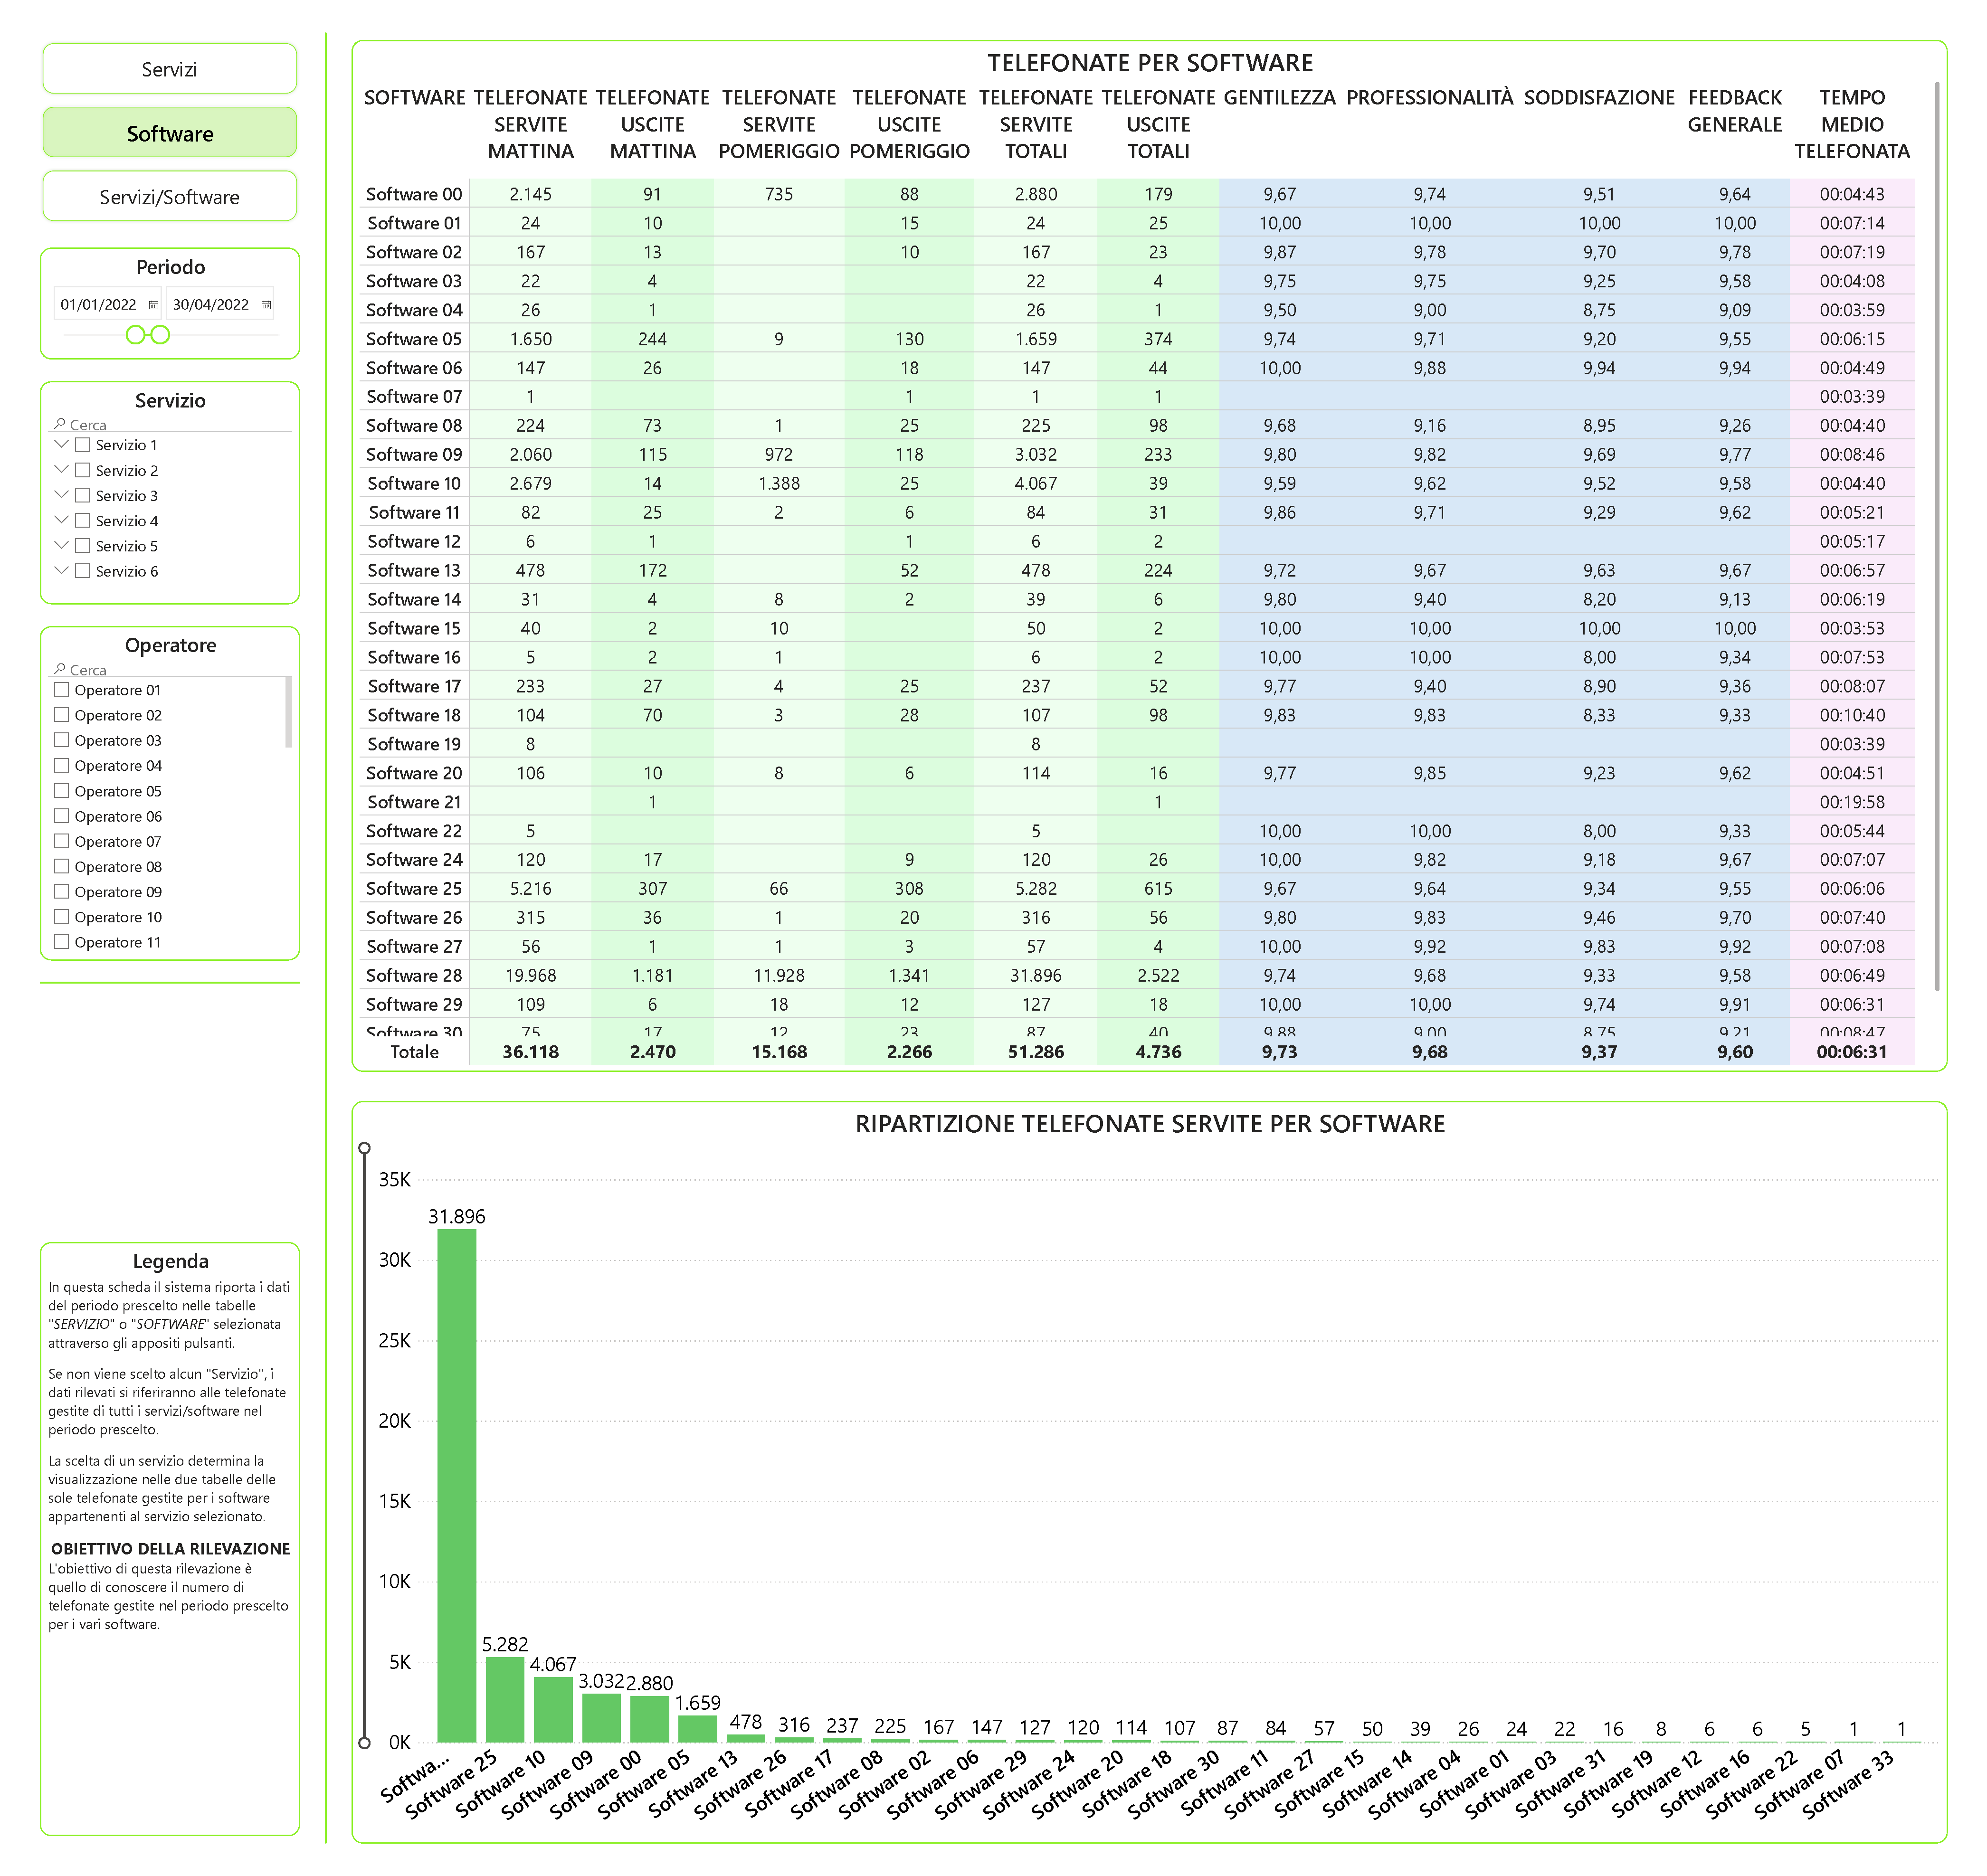
\includegraphics[height=0.9\linewidth]{figure/capitolo_4/BI Call Report-3.pdf}
        \caption{Gestite (Servizi/Software)}
        \label{fig:BI Call Report-3}
        \end{figure}
    \item \textbf{Analisi sulla gestione delle telefonate}.
        \begin{itemize}
        \item \textit{Picchi Telefonate}. Tale pagina è una dashboard con il compito di permettere di avere una visione immediata degli orari di picco, sia maggiori che minori, delle telefonate gestite e non dal reparto di supporto tecnico in modo da poter conoscere quali sono i momenti nell'arco di una giornata di minore o maggiore congestione del servizio di assistenza.
        \item \textit{Impegno periodo}. Tale pagina è una dashboard con il compito di minimizzare e far risaltare immediatamente quali sono i periodi, rispetto alla totalità delle informazioni in possesso, in cui i valori dei periodi in questione sono superiori o minori alla media generale.
        \item \textit{Riepilogo Singolo}. Tale pagina è una dashboard con la finalità di permettere di prendere visione di tutte le informazioni recuperabili dai dati, in modo conciso e chiaro, delle telefonate gestite e non dal reparto di supporto tecnico in un determinato periodo.
        \item \textit{Riepilogo Confronto}. Tale pagina è una dashboard, che evolve il ruolo della precedente dashboard, con la finalità di mettere a paragone due periodi o servizi in una singola vista e ricavare le differenze di tutte le informazioni recuperabili dai dati in possesso rispetto ai periodi in analisi.
    \end{itemize}
        \begin{figure}[H]
        \centering
        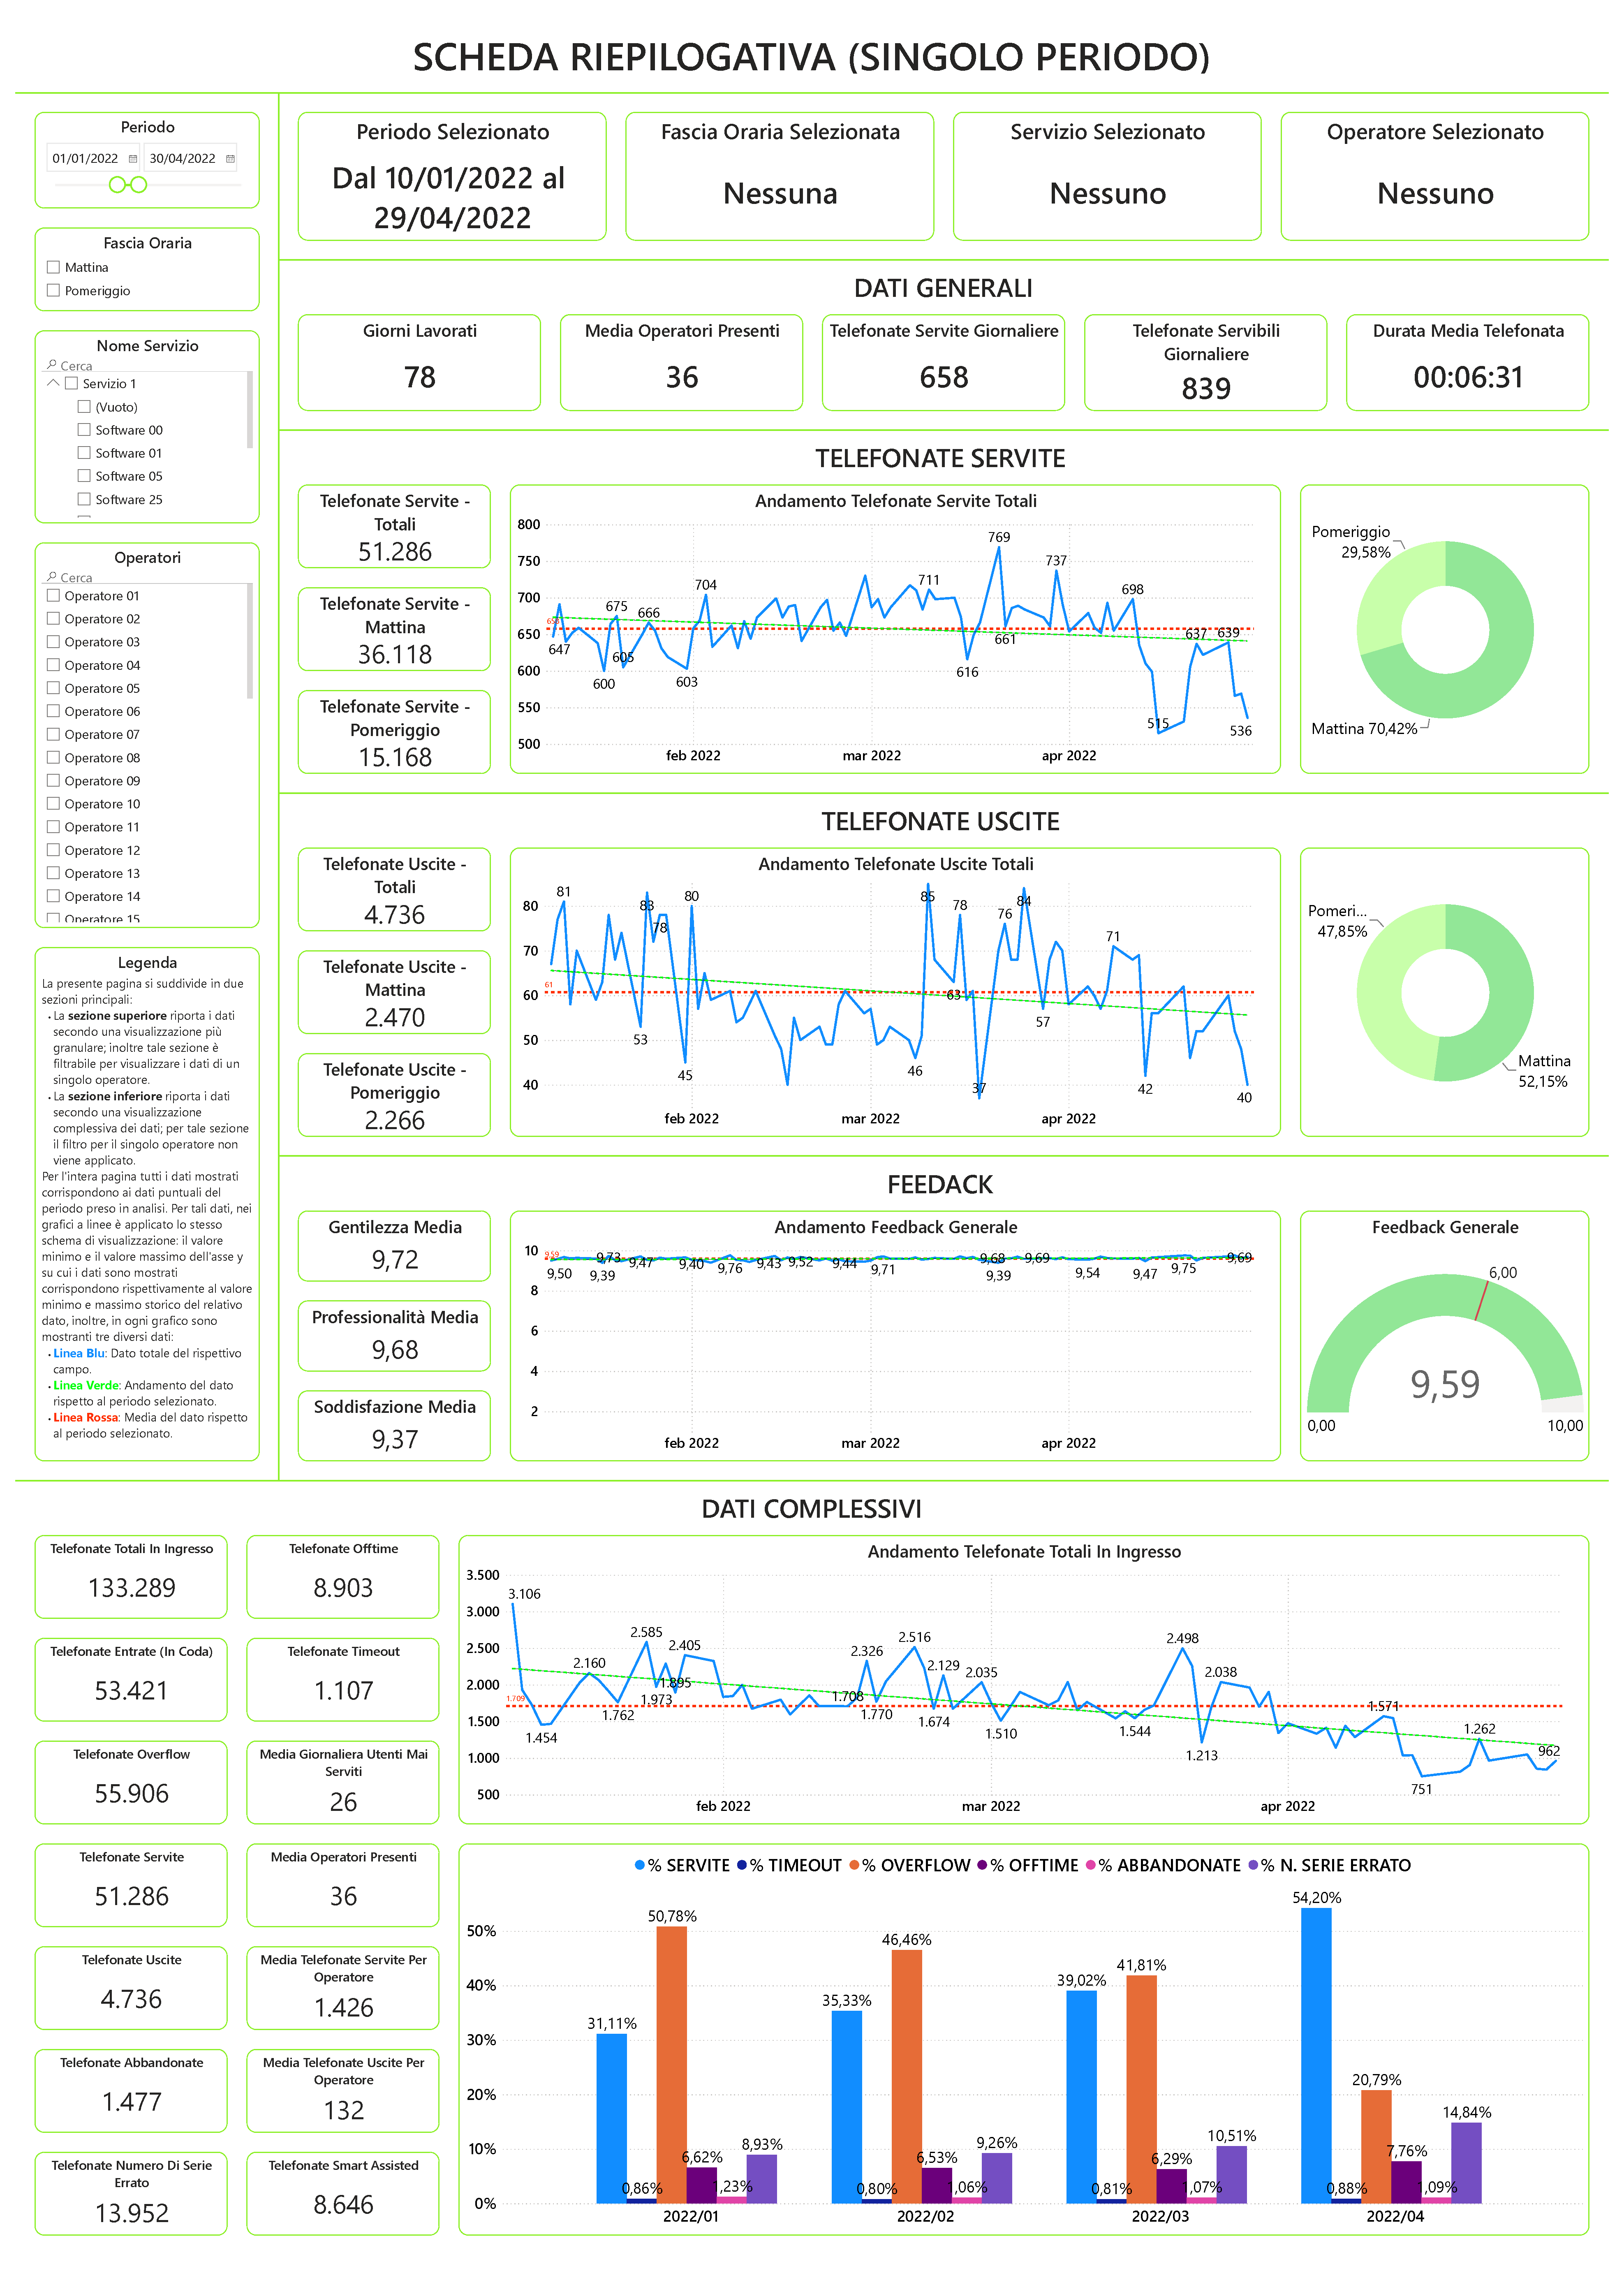
\includegraphics[height=1\linewidth]{figure/capitolo_4/BI Call Report-4.pdf}
        \caption{Riepilogo Singolo}
        \label{fig:BI Call Report-4}
        \end{figure}
\end{enumerate}

Naturalmente, ognuna delle pagine precedentemente indicate ha funzionalità di interattività con l'utente finale, il quale ha la possibilità di utilizzare filtri ad hoc per ognuna delle relative pagine in modo da poter aumentare o diminuire la granularità delle informazioni che intende visualizzare e analizzare.
Inoltre, per supportare gli utenti finali nel proprio compito, è stata definita una documentazione a cui fare riferimento dove sono indicate le finalità di ognuna delle pagine precedentemente descritte e dove è presente un glossario indicante tutte le definizioni dei termini, tecnici e non, utilizzati all'interno dell'intero sistema. Ciò permetterebbe anche ad una persona, non necessariamente addentrata all'argomento, di comprendere con maggiore facilità le finalità e le logiche adottate per le metriche mostrate.

\section{Risultati del Progetto}

Di seguito si riportano i risultati ottenuti dall'adozione del progetto precedentemente definito.

\subsection{Risultati del Data Warehousing}
Con l'implementazione del sistema di data warehousing è stato possibile centralizzare ed organizzare i dati provenienti da diverse fonti, anche di non semplice accesso, in un unico repository. Ciò ha permesso agli utenti IT oppure ai manager del reparto in questione di avere un accesso diretto e maggiormente efficiente ai dati necessari per le loro operazioni di routine. Inoltre, il sistema, come precedentemente precisato, non si è occupato unicamente di raggruppare i dati ma ha svolto anche il compito di pulizia e formattazione, rimuovendo in questo modo ogni possibile refuso o incoerenza tra i dati aventi originariamente formati differenti. Questo ha permesso di ridurre gli errori e le inconsistenze dei dati stessi e fornendo una visione più accurate e completa delle operazioni del reparto.

\subsection{Risultati della Business Intelligence}

Con l'implementazione del sistema di business intelligence sono stati apportati una serie di miglioramenti significativi nel modo in cui i decision maker del reparto di assistenza tecnica utilizzano e analizzano i dati a loro disposizione. Grazie alla creazione di appositi report e dashboard personalizzati, è stato possibile fornire una visione chiara e concisa di tutte le metriche essenziali e cruciali sull'andamento delle loro operazioni quotidiane. Per fare alcuni esempi, grazie alle rilevazioni svolte:

\begin{itemize}
    \item è stata applicata una politica di integrazione ed aumento di nuovi dipendenti che potessero svolgere il ruolo di operatori per i gruppi aventi maggiore necessità dats l'elevata richiesta di supporto rispetto il software di riferimento;
    \item è stata applicata una politica di migrazione di operatori dai gruppi che non richiedevano un elevato numero di supporto verso altri gruppi, in modo da poter bilanciare l'offerta di servizio rispetto la richiesta dei nostri clienti;
    \item è stato possibile comprendere e migliorare l'assistenza svolta da determinati operatori o per specifici servizi grazie alla rilevazione di valutazioni inferiori rispetto gli standard aziendali, così da migliorare il servizio e ricevere feedback più che positivi a seguito di tale operazione;
    \item è stato possibile svolgere una ridistribuzione delle operazioni che necessitassero di maggiore esperienza per essere eseguite tra gli utenti novizi e quelli con una maggiore maturità professionale.
\end{itemize}

In altre parole, il sistema di BI ha permesso di identificare e analizzare le tendenze e i modelli nei dati, portando ad una maggiore comprensione delle problematiche dei clienti e ha permesso al team di migliorare la qualità del servizio offerto a quest'ultimi.

\subsection{Risultati Finali}

In conclusione, l'implementazione del sistema di data warehousing e business intelligence ha portato a una serie di miglioramenti significativi nel reparto di assistenza tecnica dell'azienda. Questi miglioramenti hanno prodotto una maggiore efficienza operativa, una migliore qualità dei dati e una capacità di prendere decisioni basate sui dati perfezionata.
